\newpage
\section{Билет 13. Теоремы о вихрях в идеальной жидкости.}
\begin{center}
	\textit{\underline{Основные свойства и термины, которые будут использованы в вихревых теоремах}}
\end{center}
\begin{enumerate}
\item 
\textbf{Циркуляция векторного поля} — криволинейный интеграл, взятый по замкнутому контуру.
$$\jmath = \oint  \limits_{L}\vec{v}d\vec{l}$$
\item
\textbf{Вихревая линия} — линия, касательная к которой в каждой точке совпадает с $\vec{\omega} = \frac{1}{2}rot\vec{v}$.\\ Дифференциальное уравнение вихревой линии:
$$\frac{dx}{\omega_x} =\frac{dy}{\omega_y} = \frac{dz}{\omega_z}$$
\item 
Пусть $L$ - линия, не являющаяся вихревой. Проводя через каждую её точку вихревые линии, получаем \textbf{вихревую поверхность}. 
\item
\textbf{Вихревая трубка.}
Пусть линия $L$, не совпадающая с вихревой линией, замкнута. Если из неё выпустить вихревые линии, то полученная фигура будет называться вихревой трубкой.
\begin{figure}[!htbp]
    \begin{minipage}{0.33\linewidth}
        \centering
        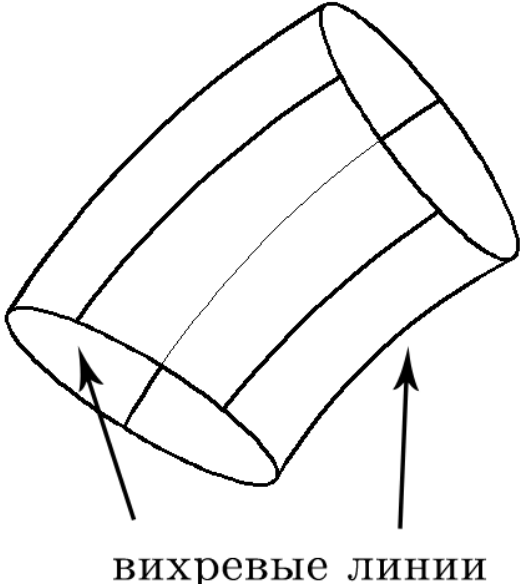
\includegraphics[width=\linewidth]{13/vihre_trubka.png}
        \captionof{figure}{Вихревая трубка}
    \end{minipage}\hfill
    \begin{minipage}{0.66\linewidth}
        \centering
        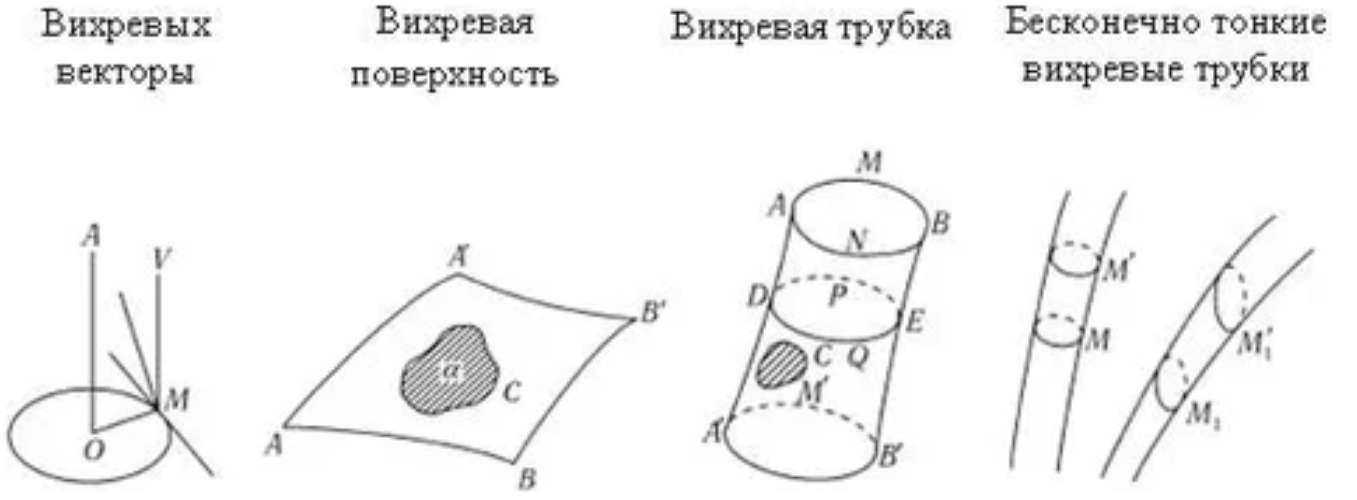
\includegraphics[width=\linewidth]{13/vihre_all.png}
        \captionof{figure}{}
    \end{minipage}
\end{figure}
\item \textbf{Интенсивность вихревой трубки} — поток ротора скорости внутри трубки через поперечное сечение $S$.
$$
\Gamma = \iint\limits_{S}\vec{\omega}d\vec{s}  =\iint\limits_{S}\vec{\omega}_nds =\text{(по теореме Стокса)} = \frac{1}{2}  \oint  \limits_{\partial S}\vec{v}d\vec{l}$$
\end{enumerate}
\begin{center}
	\textit{\underline{Уравнение эволюции завихрённости}}
\end{center}
$\vec{\omega} = \frac{1}{2}rot\vec{v} \Rightarrow div \vec{\omega}= 0$.\\
Возьмём $rot$ от уравнения движения в форме Громека-Лэмба и получим:
\begin{equation}
\label{vihre_eq_evol}
\frac{\partial \vec{\omega}}{\partial t} = rot(\vec{v}\times \vec{\omega})
\end{equation}
\begin{center}
	\textit{\underline{Первая кинематическая теорема Гельмгольца}}
\end{center}
\begin{theorem}
Интенсивность вихревой трубки одинакова по любому контуру, опоясывающему вихревую трубку.
\end{theorem}
\begin{proof}
\begin{minipage}{0.25\linewidth}
    \centering
    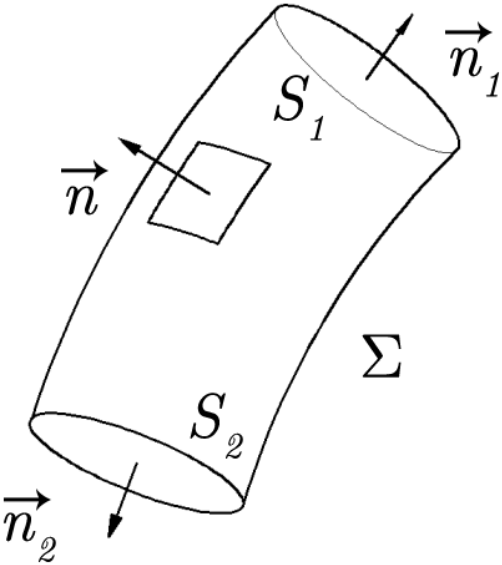
\includegraphics[width=\linewidth]{13/vihre_sech.png}
    \captionof{figure}{}
\end{minipage}
$0 = \int\limits_Vdiv \vec{\omega}dV = \int\limits_{S_1+S_2+\Sigma} \omega_ndS =\\ \text{(нормали противонаправлены и проекция\ }\omega_n \text{ на боковой поверхности, где вихревые линии, равна 0)} \\= -\int\limits_{S_1} \omega_ndS + \int\limits_{S_2} \omega_ndS + 0 = \Gamma_2 - \Gamma_1$.\\
\end{proof}
\begin{addition}
Вихревая линия получается из вихревой трубки с помощью предельного перехода при $S\xrightarrow[]{}0$.
\end{addition}
\begin{center}
	\textit{\underline{Вторая кинематическая теорема Гельмгольца}}
\end{center}
\begin{theorem}
Пусть задана вихревая трубка (или в частном случае вихревая линия). Тогда она либо замкнута, либо начинается и заканчивается на бесконечности.
\end{theorem}
\begin{proof}
(От противного) Пусть у неё есть начало, тогда в начале интенсивность нулевая. Однако из первой кинематической теоремы Гельмгольца следует, что интенсивность всюду должна быть нулевая. Противоречие.
\end{proof}
\begin{center}
	\textit{\underline{Теорема Томпсона}}
\end{center}
\begin{theorem}
В предположениях баротропности и потенциальности внешних сил выполнено соотношение \ref{vihre_eq_evol}.
Пусть линия $L$ является Лагранжевым контуром (т.е. вморожена в среду и двигается с её скоростью).
Тогда интенсивность жидкого контура остаётся постоянной.
\end{theorem}
\begin{proof}
\begin{minipage}{0.35\linewidth}
    \centering
    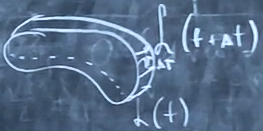
\includegraphics[width=\linewidth]{13/Tompson.png}
    \captionof{figure}{}
\end{minipage}
$\Gamma = \frac{1}{2}  \oint  \limits_{L}\vec{v}d\vec{l} = \iint\limits_{S}\vec{\omega}d\vec{s}$.\\
$$\frac{d\Gamma}{dt} =
\lim\limits_{\Delta t \xrightarrow[]{} 0} \frac{
\oint  \limits_{L(t + \Delta t)}\vec{v}(\vec{r}, t + \Delta t)d\vec{l}
-
\oint  \limits_{L(t)}\vec{v}(\vec{r}, t)d\vec{l}
}{\Delta t}
=
\lim\limits_{\Delta t \xrightarrow[]{} 0} \frac{\Gamma(t+\Delta t) - \Gamma(t)}{\Delta t}.
$$

$$0 = \int\limits_Vdiv \vec{\omega}dV = -\int\limits_{S(t)} \vec{\omega}(\vec{r}, t) d\vec{S} + \int\limits_{S(t+\Delta t)} \vec{\omega}(\vec{r}, t) d\vec{S} + \int\limits_{S_{\text{бок}}} \vec{\omega}(\vec{r}, t) d\vec{S} \Rightarrow [d\vec{S} = d\vec{l}\times \vec{v}\Delta t] \Rightarrow$$
$$\Rightarrow 
\Gamma(t) = \int\limits_{S(t+\Delta t)} \vec{\omega}(\vec{r}, t) d\vec{S} + \oint\limits_{L} \vec{\omega}(\vec{r}, t)[d\vec{l}\times \vec{v}]\Delta t \Rightarrow \\$$
$$\Rightarrow  
\frac{d\Gamma}{dt} =
\lim\limits_{\Delta t \xrightarrow[]{} 0} \frac{
\int  \limits_{S(t + \Delta t)}[\vec{\omega}(\vec{r}, t + \Delta t) - \vec{\omega}(\vec{r}, t)]dS
-
\oint\limits_{L} \vec{\omega}(\vec{r}, t)[d\vec{l}\times \vec{v}]\Delta t
}{\Delta t}
=$$
$$=
\int\limits_S \frac{\partial\vec{\omega}}{\partial t}dS - \oint\limits_{L} \vec{\omega}(\vec{r}, t)[d\vec{l}\times \vec{v}] =$$
$$=
\int\limits_S \frac{\partial\vec{\omega}}{\partial t}dS - \oint\limits_{L} d\vec{l}[\vec{v}\times \vec{\omega}] = \text{(т. Стокса)} = \int\limits_S (\frac{\partial\vec{\omega}}{\partial t} - rot[\vec{v}\times\vec{\omega}])dS = 0,$$
$\text{\ в силу уравнения \ref{vihre_eq_evol} и произвольности контура.}
$
\end{proof}
\begin{center}
	\textit{\underline{Следствия теоремы Томпсона. Динамическая теорема Гельмгольца.Теорема Лагранжа.}}
\end{center}
\begin{theorem}
В условиях предыдущей теоремы пусть задана вихревая поверхность. Тогда при движении вихревая поверхность переходит в вихревую поверхность.
\end{theorem}
\begin{proof}
Для любого жидкого контура на этой поверхности интенсивность равна нулю (т.к. $\omega_n = 0$).\\
При движении интенсивность отаётся нулём. Значит, переходим в вихревую поверхность.
\end{proof}
\begin{addition}
Аналогично для вихревой линии и вихревой трубки.
\end{addition}
\begin{theorem}
В условиях предыдущей теоремы. Если в начальный момент времени $t_0$ отсутствовали вихри (движение потенциально), то их не будет и для любого $t_0 + \Delta t$ (движение всё ещё потенциально).
\end{theorem}
\begin{proof}
$\Gamma = 0, t = t_0 \Rightarrow \Gamma = 0,\ \forall t.$
\end{proof}
